\subsection{VHDL model}
At the input and output of the filter there are registers to synchronize the data with the clock and two validation signals for the data, $VIN$ and $VOUT$. In \autoref{fig:IIR_1} is shown the filter architecture, where the input and output registers have been neglected, the form used is the direct form II. The sampled input data enter from the $x[n]$ port, are processed and the results exit from the $y[n]$ port. The internal parallelism of the machine is different from the external one, to avoid the possibility of overflow with any combination of input data when summing, the precision has been extended to 12 bits by extending the sign to all input signals. The multiplier, on the other hand, has no problems of parallelism because it is possible to have sufficient precision by truncating the less significant bits at each multiplication and therefore having the same parallelism between input and output data. The internal register of the machine has an enable signal which is managed by the input data validation signal so that when invalid data is received, it does not sample keeping the correct output data.

\begin{figure}[h]
	\center
	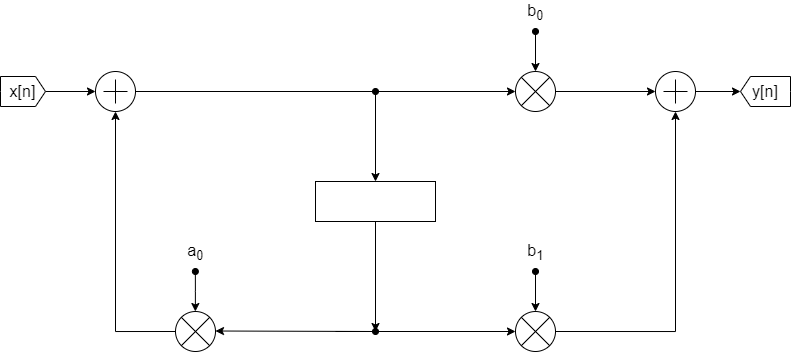
\includegraphics[width=0.8\textwidth]{iir_1.png}
	\caption{IIR filter architecture}
	\label{fig:IIR_1}
\end{figure}